\documentclass[11pt]{article}
\usepackage{tikz}
\usepackage{amssymb}
\usepackage{geometry}
\geometry{letterpaper, landscape, margin=0.4in}
\usetikzlibrary{positioning, calc, decorations.pathmorphing}

\begin{document}

\begin{center}
{\Huge \textbf{THE SILO DEPTHS}}\\[0.3em]
{\Large Level 3B --- Illaktamus \& Natural Caverns | 10 Keyed Areas}
\end{center}

\vspace{0.3em}

\begin{center}
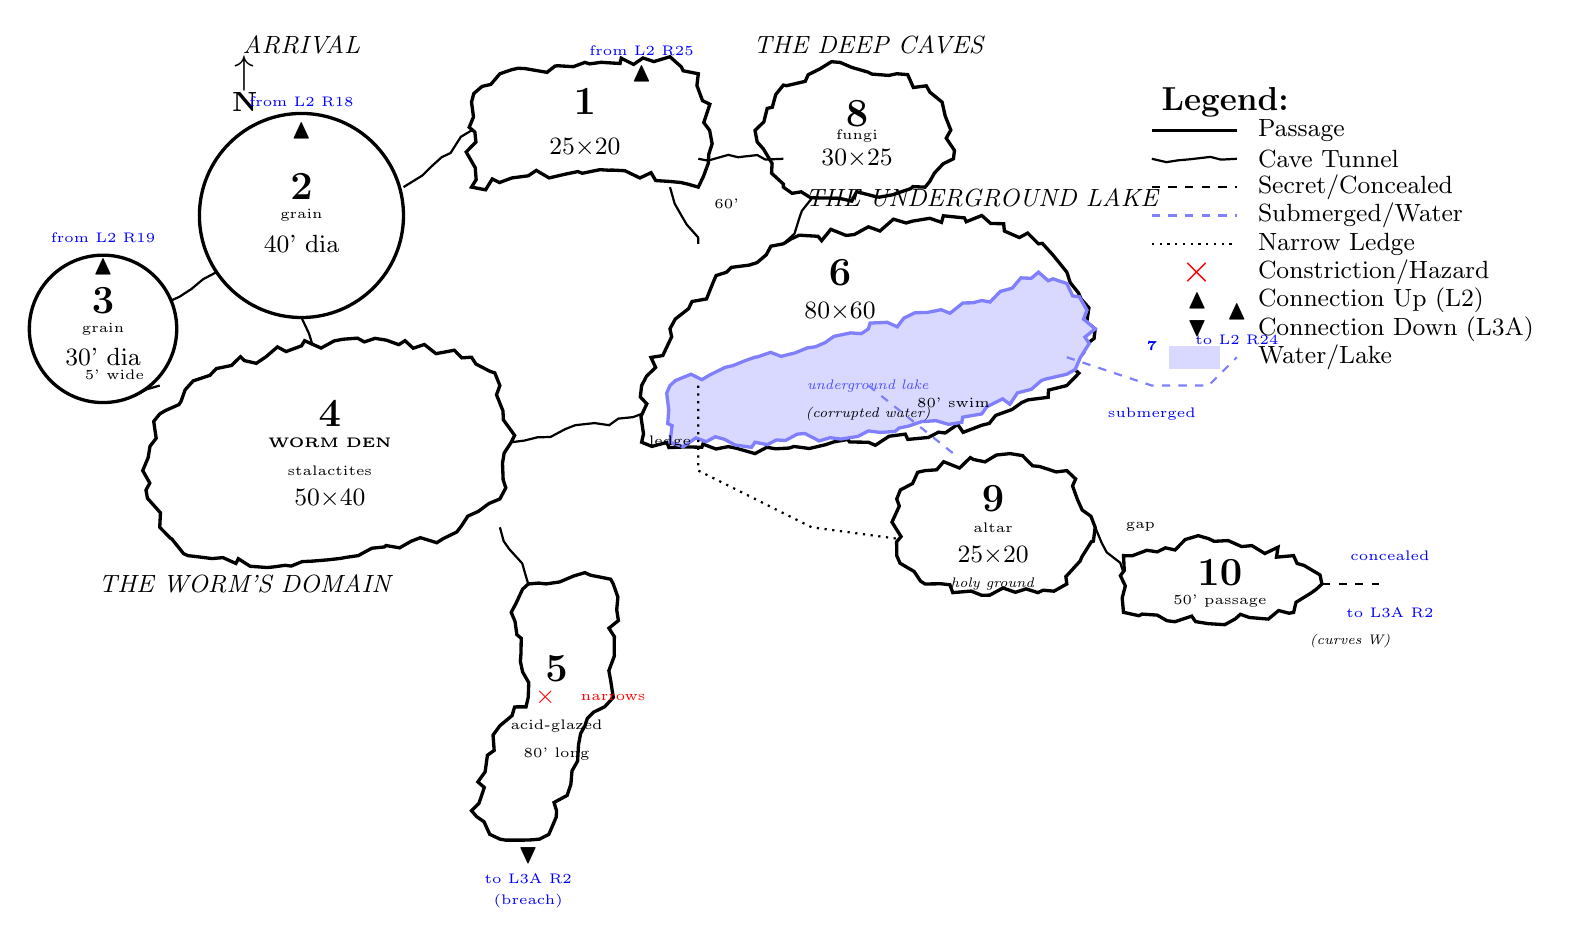
\begin{tikzpicture}[
    room/.style={draw, very thick},
    cave/.style={draw, very thick, decorate, decoration={random steps, segment length=4pt, amplitude=2pt}},
    connection/.style={draw, thick},
    cavepath/.style={draw, thick, decorate, decoration={random steps, segment length=5pt, amplitude=1.5pt}},
    water/.style={fill=blue!15, draw=blue!50, very thick, decorate, decoration={random steps, segment length=4pt, amplitude=2pt}},
    door/.style={fill=white, draw=black, thick},
    secret/.style={dashed, thick},
    scale=0.72
]

% ============================================================
% NORTH ARROW
% ============================================================
\node at (-5,11) {\Large $\uparrow$};
\node at (-5,10.5) {\textbf{N}};

% ============================================================
% ARRIVAL (Rooms 1-3) --- top of map
% ============================================================

% Room 1: The Bone Stair Landing (25x20, irregular)
\draw[cave] (-1,9) -- (0,9.2) -- (1.5,9.3) -- (2.5,9.1) -- (3,9) -- (3.2,10) -- (3,11) -- (2.5,11.3) -- (1,11.2) -- (-0.5,11) -- (-1,10.5) -- cycle;
\node at (1,10.5) {\Large \textbf{1}};
\node[font=\small] at (1,9.7) {25$\times$20};
\node at (2,11) {$\blacktriangle$};
\node[font=\tiny,blue] at (2,11.4) {from L2 R25};

% Room 2: The Grain Chute (40' dia circular)
\draw[very thick] (-4,8.5) circle (1.8);
\node at (-4,9) {\Large \textbf{2}};
\node[font=\small] at (-4,8) {40' dia};
\node at (-4,10) {$\blacktriangle$};
\node[font=\tiny,blue] at (-4,10.5) {from L2 R18};
\node[font=\tiny] at (-4,8.5) {grain};

% Room 3: The East Shaft Floor (30' dia circular)
\draw[very thick] (-7.5,6.5) circle (1.3);
\node at (-7.5,7) {\Large \textbf{3}};
\node[font=\small] at (-7.5,6) {30' dia};
\node at (-7.5,7.6) {$\blacktriangle$};
\node[font=\tiny,blue] at (-7.5,8.1) {from L2 R19};
\node[font=\tiny] at (-7.5,6.5) {grain};

% ============================================================
% Connections between Rooms 1-3
% ============================================================

% Connection 1->2 (west, 40' passage)
\draw[cavepath] (-1,10) -- (-2.2,9);

% Connection 2->3 (southwest, 30' passage through cave)
\draw[cavepath] (-5.5,7.5) -- (-6.3,7);

% ============================================================
% THE WORM'S DOMAIN (Rooms 4-5)
% ============================================================

% Room 4: The Worm Den (50x40, large irregular)
\draw[cave] (-6,2.5) -- (-4.5,2.3) -- (-3,2.5) -- (-1.5,2.8) -- (-0.5,3.5) -- (-0.3,4.5) -- (-0.5,5.5) -- (-1,6) -- (-2.5,6.3) -- (-4,6.2) -- (-5.5,5.8) -- (-6.5,5) -- (-6.8,4) -- (-6.5,3) -- cycle;
\node at (-3.5,5) {\Large \textbf{4}};
\node[font=\small] at (-3.5,3.5) {50$\times$40};
\node[font=\tiny] at (-3.5,4.5) {\textbf{WORM DEN}};
\node[font=\tiny] at (-3.5,4) {stalactites};

% Connection 2->4 (south, 20' wide tunnel)
\draw[cavepath] (-4,6.7) -- (-3.8,6.2);

% Connection 3->4 (south, 5' narrow passage)
\draw[cavepath] (-7,5.3) -- (-6.5,5.5);
\node[font=\tiny] at (-7.3,5.7) {5' wide};

% Room 5: The Acid-Bored Tunnel (10' wide, 80' long)
\draw[cave] (0,2) -- (1,2.2) -- (1.5,2) -- (1.5,0) -- (1,-0.5) -- (0.5,-2) -- (0.2,-2.5) -- (-0.5,-2.5) -- (-1,-2) -- (-0.5,-0.5) -- (0,0) -- (-0.3,1.5) -- cycle;
\node at (0.5,0.5) {\Large \textbf{5}};
\node[font=\tiny] at (0.5,-0.5) {acid-glazed};
\node[font=\tiny] at (0.5,-1) {80' long};

% Connection 4->5 (south)
\draw[cavepath] (-0.5,3) -- (0,2);

% Exit from Room 5 to Level 3A Room 2
\node at (0,-2.8) {$\blacktriangledown$};
\node[font=\tiny,blue] at (0,-3.2) {to L3A R2};
\node[font=\tiny,blue] at (0,-3.6) {(breach)};

% Constriction point marker
\node[red] at (0.3,0) {\small $\times$};
\node[font=\tiny,red] at (1.5,0) {narrows};

% ============================================================
% THE UNDERGROUND LAKE (Rooms 6-7)
% ============================================================

% Room 6: The Lakeshore Cavern (80x60, largest room)
% Shore area (north)
\draw[cave] (2,4.5) -- (4,4.3) -- (6,4.5) -- (8,4.8) -- (9.5,5.5) -- (10,6.5) -- (9.5,7.5) -- (9,8) -- (8,8.5) -- (6,8.3) -- (4.5,8) -- (3.5,7.5) -- (2.5,6.5) -- (2,5.5) -- cycle;
% Lake water fill
\draw[water] (2.5,4.5) -- (4,4.5) -- (6,4.7) -- (8,5) -- (9.5,5.7) -- (10,6.5) -- (9.5,7.3) -- (9,7.5) -- (8,7) -- (6,6.5) -- (4,6) -- (2.5,5.5) -- cycle;
\node at (5.5,7.5) {\Large \textbf{6}};
\node[font=\small] at (5.5,6.8) {80$\times$60};
\node[font=\tiny,blue!70] at (6,5.5) {\textit{underground lake}};
\node[font=\tiny] at (6,5) {\textit{(corrupted water)}};

% Connection 1->6 (south, 60' descending tunnel)
\draw[cavepath] (2.5,9) -- (3,8);
\node[font=\tiny] at (3.5,8.7) {60'};

% Connection 4->6 (east, 15' passage ascending)
\draw[cavepath] (-0.3,4.5) -- (2,5);

% Room 7: The Drowned Passage (submerged, shown as dashed)
\draw[thick,dashed,blue!50] (9.5,6) -- (11,5.5) -- (12,5.5) -- (12.5,6);
\node[font=\tiny,blue] at (11,6.2) {\textbf{7}};
\node[font=\tiny,blue] at (11,5) {submerged};
\node[font=\tiny,blue] at (12.5,6.3) {to L2 R24};
\node at (12.5,6.8) {$\blacktriangle$};

% ============================================================
% THE DEEP CAVES (Rooms 8-10)
% ============================================================

% Room 8: The Fungal Grotto (30x25)
\draw[cave] (4.5,9) -- (5.5,8.8) -- (7,9) -- (7.5,9.5) -- (7.3,10.5) -- (6.5,11) -- (5.5,11.2) -- (4.5,10.8) -- (4,10) -- cycle;
\node at (5.8,10.3) {\Large \textbf{8}};
\node[font=\small] at (5.8,9.5) {30$\times$25};
\node[font=\tiny] at (5.8,9.9) {fungi};

% Connection 1->8 (southeast, 30' passage)
\draw[cavepath] (3,9.5) -- (4.5,9.5);

% Connection 8->6 (west/south, 20' passage along shore)
\draw[cavepath] (5,8.8) -- (4.5,8);

% Room 9: The Collapsed Shrine (25x20, on far side of lake)
\draw[cave] (7,2) -- (8,1.8) -- (9.5,2) -- (10,3) -- (9.5,4) -- (8.5,4.3) -- (7,4) -- (6.5,3.5) -- (6.5,2.5) -- cycle;
\node at (8.2,3.5) {\Large \textbf{9}};
\node[font=\small] at (8.2,2.5) {25$\times$20};
\node[font=\tiny] at (8.2,3) {altar};
\node[font=\tiny] at (8.2,2) {\textit{holy ground}};

% Connection 6->9 (across lake, 80' swim)
\draw[thick,dashed,blue!50] (6,5.5) -- (7.5,4.3);
\node[font=\tiny] at (7.5,5.2) {80' swim};
% Narrow ledge along west wall
\draw[thick,dotted] (3,5.5) -- (3,4) -- (5,3) -- (6.5,2.8);
\node[font=\tiny] at (2.5,4.5) {ledge};

% Room 10: The Passage to the Sanctum (10' wide, 50' long)
\draw[cave] (10.5,1.5) -- (12,1.3) -- (13.5,1.5) -- (14,2) -- (13.5,2.5) -- (12,2.8) -- (10.5,2.5) -- cycle;
\node at (12.2,2.2) {\Large \textbf{10}};
\node[font=\tiny] at (12.2,1.7) {50' passage};

% Connection 9->10 (west/east, through rockfall gap)
\draw[cavepath] (10,3) -- (10.5,2.2);
\node[font=\tiny] at (10.8,3) {gap};

% Exit to Level 3A Room 2 (concealed door, passage curves west)
\draw[thick,dashed] (14,2) -- (15,2);
\node[font=\tiny,blue] at (15.2,2.5) {concealed};
\node[font=\tiny,blue] at (15.2,1.5) {to L3A R2};
\node[font=\tiny] at (14.5,1) {\textit{(curves W)}};

% ============================================================
% WING LABELS
% ============================================================
\node[font=\small\itshape] at (-4,11.5) {ARRIVAL};
\node[font=\small\itshape] at (-5,2) {THE WORM'S DOMAIN};
\node[font=\small\itshape] at (6,11.5) {THE DEEP CAVES};
\node[font=\small\itshape] at (8,8.8) {THE UNDERGROUND LAKE};

% ============================================================
% LEGEND
% ============================================================
\node[anchor=west,font=\large] at (11,10.5) {\textbf{Legend:}};

\draw[thick] (11,10) -- (12.5,10);
\node[anchor=west,font=\small] at (12.7,10) {Passage};

\draw[cavepath] (11,9.5) -- (12.5,9.5);
\node[anchor=west,font=\small] at (12.7,9.5) {Cave Tunnel};

\draw[thick,dashed] (11,9) -- (12.5,9);
\node[anchor=west,font=\small] at (12.7,9) {Secret/Concealed};

\draw[thick,dashed,blue!50] (11,8.5) -- (12.5,8.5);
\node[anchor=west,font=\small] at (12.7,8.5) {Submerged/Water};

\draw[thick,dotted] (11,8) -- (12.5,8);
\node[anchor=west,font=\small] at (12.7,8) {Narrow Ledge};

\node[red] at (11.8,7.5) {\Large $\times$};
\node[anchor=west,font=\small] at (12.7,7.5) {Constriction/Hazard};

\node at (11.8,7) {$\blacktriangle$};
\node[anchor=west,font=\small] at (12.7,7) {Connection Up (L2)};

\node at (11.8,6.5) {$\blacktriangledown$};
\node[anchor=west,font=\small] at (12.7,6.5) {Connection Down (L3A)};

\fill[blue!15] (11.3,5.8) rectangle (12.2,6.2);
\node[anchor=west,font=\small] at (12.7,6) {Water/Lake};

\end{tikzpicture}
\end{center}

\vspace{0.5em}

\section*{Room Key}
\begin{small}
\begin{tabular}{rl|rl}
1 & Bone Stair Landing (25$\times$20) & 6 & Lakeshore Cavern (80$\times$60) \\
2 & Grain Chute (40' dia) & 7 & Drowned Passage (submerged) \\
3 & East Shaft Floor (30' dia) & 8 & Fungal Grotto (30$\times$25) \\
4 & The Worm Den (50$\times$40) & 9 & Collapsed Shrine (25$\times$20) \\
5 & Acid-Bored Tunnel (80' long) & 10 & Passage to Sanctum $\rightarrow$ L3A \\
\end{tabular}
\end{small}

\section*{Connections to Other Levels}
\begin{small}
\begin{itemize}
    \item \textbf{Room 1 (Bone Stair Landing):} Stairs up to Level 2, Room 25 (Bone Stair).
    \item \textbf{Room 2 (Grain Chute):} Silo shaft up to Level 2, Rooms 22/18 (30' climb through grain).
    \item \textbf{Room 3 (East Shaft Floor):} Silo shaft up to Level 2, Rooms 22/19 (30' climb through grain).
    \item \textbf{Room 5 (Acid-Bored Tunnel):} Worm breach south to Level 3A, Room 2 (Pilgrim's Stair).
    \item \textbf{Room 7 (Drowned Passage):} Submerged tunnel east to Level 2, Room 24 (Flooded Cistern).
    \item \textbf{Room 10 (Passage to Sanctum):} Concealed door west to Level 3A, Room 2 (Pilgrim's Stair).
\end{itemize}
\end{small}

\end{document}
